\chapter{Angles}

In the videos I'm about to recommend, the narrator will talk about
lines, line segments, and rays. When mathematicians talk about
\emph{lines}, they mean a straight line that goes forever in both
directions. Pick any two points on a line; the points between them are
a \emph{line segment}. If you take any line, pick a point on that line
and discard all the points on one side of the point, that is a
\emph{ray}. All three are infinitely thin.

\begin{tikzpicture}[scale=1.5]
  \coordinate (a) at (-0.3, -0.6);
  \coordinate (d) at (1.3, 2.6);
  \draw [<->](a)--node [right]{"Line"}(d);
\end{tikzpicture}
\hspace{10mm}
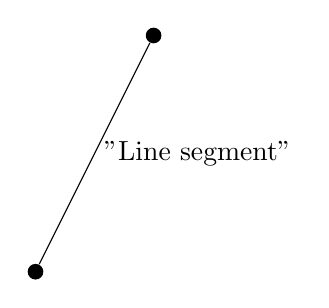
\begin{tikzpicture}[scale=1.5]
  \coordinate [circle, fill, inner sep=2pt] (b) at (0,0) ;
  \coordinate [circle, fill, inner sep=2pt] (c) at (1, 2) ;
  \draw (b)--node [right]{"Line segment"}(c);
\end{tikzpicture}
\hspace{6mm}
\begin{tikzpicture}[scale=1.5]
  \coordinate [circle, fill, inner sep=2pt] (b) at (0,0) ;
  \coordinate (d) at (1.3, 2.6);
  \coordinate (lab) at (0.8, 1.0);
  \draw [->](b)--node[right] {"Ray"} (d)  ;
\end{tikzpicture}


Watch the following videos from Khan Academy:
\begin{itemize}
\item Introduction to angles: \url{https://youtu.be/H-de6Tkxej8}
\item Measuring angles in degrees: \url{https://youtu.be/92aLiyeQj0w} 
\end{itemize}

When two lines cross, they form four angles:

\begin{tikzpicture}[scale=3]
  \coordinate (a) at (0, 1.5);
  \coordinate (b) at (1.6, 2);
  \coordinate (c) at (1.6, 1.5);
  \coordinate (d) at (0, 1);
  \coordinate [circle, fill, inner sep=1pt](e) at (0.8, 1.5) ;
  \draw [->](e)--(a) node[left] {$A$}  ;
  \draw [->](e)--(b) node[right] {$B$}  ;
  \draw [->](e)--(c) node[right] {$C$}  ;
  \draw [->](e)node[above]{$E$}--(d) node[left] {D} ;
  \pic [draw, <->, "$\scriptstyle  \angle AEB$ ", angle radius = 0.8cm, angle eccentricity=1.3] {angle = b--e--a};
  \pic [draw, <->, "$\scriptstyle  \angle BEC$ ", angle radius = 1.1cm, angle eccentricity = 1.5] {angle = c--e--b};
  \pic [draw, <->, "$\scriptstyle  \angle CED$ ", angle radius = 0.8cm, angle eccentricity=1.3] {angle = d--e--c};
  \pic [draw, <->, "$\scriptstyle  \angle DEA$ ", angle radius = 1.1cm, angle eccentricity=1.5] {angle = a--e--d};
\end{tikzpicture}

What do we know about those angles?
\begin{itemize}
\item The sum of any two adjacent angles add to be $180^\circ$.  So, for example, $m \angle AEB + m \angle BEC = 180^\circ$. We use the phrase ``add to be $180^{\circ}$'' so often that we have a special word for it: We say that two angles are \emph{supplementary} if they add to be $180^\circ$.
\item The sum of all four angles is $360^\circ$.
\item Angles opposite each other are equal. So, for example, $m \angle AEB = m \angle CED$.
\end{itemize}

In a diagram, when we want to indicate that two angles are equal, we often put hash marks in the angle:

\begin{tikzpicture}[scale=3]
  \coordinate (a) at (0, 1.5);
  \coordinate (b) at (1.6, 2);
  \coordinate (c) at (1.6, 1.5);
  \coordinate (d) at (0, 1);
  \coordinate [circle, fill, inner sep=1pt](e) at (0.8, 1.5) ;
  \draw [->](e)--(a) node[left] {$A$}  ;
  \draw [->](e)--(b) node[right] {$B$}  ;
  \draw [->](e)--(c) node[right] {$C$}  ;
  \draw [->](e)node[above]{$E$}--(d) node[left] {D} ;
  \tkzMarkAngle[size = 0.2cm,mark = |](b,e,a)
  \tkzMarkAngle[size = 0.3cm,mark = ||](c,e,b)
  \tkzMarkAngle[size = 0.2cm,mark = |](d,e,c)
  \tkzMarkAngle[size = 0.3cm,mark = ||](a,e,d)
\end{tikzpicture}

Here the two angles with a single hash mark are equal and the two angles with double hash marks are equal.

When two lines are perpendicular, the angle between them is $90^\circ$ and we say they meet at a \emph{right angle}. When drawing diagrams, we indicate right angles with an elbow:

\begin{tikzpicture}[scale=1.5]
  \coordinate (a) at (0, 1.5);
  \coordinate (b) at (0, 0);
  \coordinate (c) at (1.5, 0);
  \draw [->](b)--(a)  ;
  \draw [->](b)--(c)  ;
  \pic [draw,thick,angle eccentricity=.5]{right angle = a--b--c};
\end{tikzpicture}
 
When an angle is less than $90^\circ$, it is said to be
\emph{acute}. When an angle is more than $90^\circ$, it is said to be
\emph{obtuse}.

\begin{tikzpicture}[scale=3]
  \coordinate (a) at (0.4, 0.6);
  \coordinate (b) at (0, 0);
  \coordinate (c) at (0.9, 0);
  \draw [->](b)--(a)  ;
  \draw [->](b)--(c)  ;
  \pic [draw, <->, "acute", angle radius = 1cm, angle eccentricity=1.5] {angle = c--b--a};
  \end{tikzpicture}
\hspace{2cm}
\begin{tikzpicture}[scale=3]
  \coordinate (a) at (1, 0.6);
  \coordinate (b) at (0.5, 0);
  \coordinate (c) at (0, 0);
  \draw [->](b)--(a)  ;
  \draw [->](b)--(c)  ;
  \pic [draw, <->, "obtuse", angle radius = 0.6cm, angle eccentricity=1.5] {angle = a--b--c};
\end{tikzpicture}

If two lines are parallel, line segments that intersect both form the same angles:

\begin{tikzpicture}[scale=3]
  \coordinate (a) at (0, 1);
  \coordinate [circle, fill, inner sep=1pt](b) at (1.5, 1.5);
  \coordinate (c) at (1.5, 1);
  \coordinate (d) at (0.5, 0.5);
  \coordinate (e) at (1, 1);
  \coordinate (f) at (0, 0.5);
  \coordinate (g) at (1.5, 0.5);
  \coordinate [circle, fill, inner sep=1pt](h) at (0, 0);
  \draw [->](e)--(a);
  \draw [-](e)--(b);
  \draw [->](e)--(c);
  \draw [-](e)--(d);
   \draw [->](d)--(f);
  \draw [->](d)--(g);
  \draw [-](d)--(h);
  \tkzMarkAngle[size = 0.15cm,mark = |](b,e,a)
  \tkzMarkAngle[size = 0.2cm,mark = ||](c,e,b)
  \tkzMarkAngle[size = 0.15cm,mark = |](d,e,c)
  \tkzMarkAngle[size = 0.2cm,mark = ||](a,e,d)
  
   \tkzMarkAngle[size = 0.15cm,mark = |](e,d,f)
  \tkzMarkAngle[size = 0.2cm,mark = ||](g,d,e)
  \tkzMarkAngle[size = 0.15cm,mark = |](h,d,g)
  \tkzMarkAngle[size = 0.2cm,mark = ||](f,d,h)
\end{tikzpicture}



